\documentclass{beamer}
% \usepackage{lmodern}
%=====================================================================
% Color definition
\definecolor{jvagreen}{RGB}{0,104,	139}
\definecolor{jvagold}{RGB}{255, 255, 255}
\setbeamercolor{section in head/foot}{fg = jvagold, bg = jvagreen}
\usepackage{graphicx}
\usepackage{mathtools}
\usepackage{picture}
\usepackage{amsmath}
\usepackage{multimedia}
\DeclareMathOperator{\Tr}{Tr}
\graphicspath{{../}}
%\setbeameroption{show notes}
\usepackage{multicol}
\usepackage{multirow}
\usepackage{caption}
\usepackage{textpos}
\setbeamercovered{dynamic}
\usepackage[makeroom]{cancel}
\usepackage{natbib}


% Common math symbols used in the presentation
\newcommand{\phim}{\mathbf{\phi}}
\newcommand{\X}{\mathbf{X}}
\newcommand{\x}{\mathbf{x}}
\newcommand{\Y}{\mathbf{Y}}
\newcommand{\y}{\mathbf{y}}
\newcommand{\w}{\mathbf{w}}
\newcommand{\Z}{\mathbf{Z}}
\newcommand{\z}{\mathbf{z}}
\newcommand{\h}{\mathbf{h}}
\newcommand{\omegam}{\boldsymbol{\omega}}
\newcommand{\deltax}{\left \|  \Delta \x \right \|}
\newcommand{\lxo}{\lambda, \x, \omegam}
\newcommand{\C}{\,^{\circ}{\rm C}}
\newcommand{\Maya}{Maya\textsuperscript\textregistered~}
\newcommand{\MentalRay}{Mental Ray\textsuperscript\textregistered~}
\newcommand{\Matlab}{Matlab\textsuperscript\textregistered~}

\usebackgroundtemplate
{
    
\includegraphics[width=\paperwidth,height=\paperheight]{img/blank.jpg}%
}
\beamertemplatenavigationsymbolsempty

%=====================================================================
% Templates - headline, frametitle

\makeatletter
% Komprimiert die miniframe Kreise auf eine Linie
\beamer@compresstrue
\makeatother

% Definiert die headline
\setbeamertemplate{headline}
{ 
%\includegraphics[width=\paperwidth]{pic} % test logo
\begin{beamercolorbox}[wd=\paperwidth,right]{section in head/foot}
    \rule{\paperwidth}{1pt}
    %Vertikaler Abstand
    \vskip20pt
    %Fügt die Standard-Navi ein (miniframes)
    %\insertnavigation{\paperwidth}
    \vskip8pt
    %\rule{\paperwidth}{0.5pt}
    %\vskip25.5pt % same height of the example provided, but IMHO is too much
    \rule{\paperwidth}{1pt}
\end{beamercolorbox} 
}
\setbeamertemplate{footline}
{ 
%\includegraphics[width=\paperwidth]{pic} % test logo
\begin{beamercolorbox}[wd=\paperwidth,right]{section in head/foot}
    \rule{\paperwidth}{1pt}
    %Vertikaler Abstand
    \vskip10pt
    %Fügt die Standard-Navi ein (miniframes)
    \insertnavigation{\paperwidth}
    \vskip8pt
    \rule{\paperwidth}{0.5pt}
    %\vskip25.5pt % same height of the example provided, but IMHO is too much
    %\rule{\paperwidth}{1pt}
\end{beamercolorbox} 
}

% definition of the frametitle
\setbeamertemplate{frametitle}
{
\vskip-24pt % to shift up the frametitle
\hbox{ 
 \begin{beamercolorbox}[wd=.0675\textwidth]{} % left shift
 \end{beamercolorbox} 
 \begin{beamercolorbox}[sep=4pt]{section in head/foot}
 \insertframetitle
 \end{beamercolorbox} 
 }
}

\mode<presentation>
{
    \setbeamertemplate{itemize item}[circle]
    \setbeamercolor{itemize item}{fg = jvagreen}
    \setbeamertemplate{itemize subitem}[circle]
    \setbeamercolor{itemize subitem}{fg = jvagreen}
}

\renewcommand\footnoterule{}

\AtBeginSection[]
{
  \begin{frame}<beamer>
    \frametitle{Outline}
    \tableofcontents[currentsection]
  \end{frame}
}

%\logo{\includegraphics[height=0.6cm]{img/cde_basic_green}}
%\let\oldequation=\equation
%\let\endoldequation=\endequation
%\renewenvironment{equation}{\vspace{1cm}\begin{oldequation}}{\end{oldequation}\vspace{15mm}}

\begin{document}

\addtobeamertemplate{frametitle}{}{%
\begin{textblock*}{100mm}(-0.9cm,-0.6cm)

\includegraphics[height=0.5cm,width=1.5cm]{img/uob-logo-white-transparent}
\end{textblock*}
\begin{textblock*}{100mm}(0.98\textwidth,-0.6cm)

\includegraphics[height=0.5cm,width=1cm]{img/cde_tag_white}
\end{textblock*}
}

\title[Realistic fire rendering]{
 Realistic fire rendering}

% Optional: a subtitle to be dispalyed on the title slide
% \subtitle{Show where you're from}
% \subtitle{Presented by: Ieva Kazlauskaite}
% The author(s) of the presentation:
%  - again first a short version to be displayed at the bottom;
%  - next the full list of authors, which may include contact information;
\author[Garoe Dorta Perez]{
   Garoe Dorta Perez } 


% The institute:
%  - to start the name of the university as displayed on the top of each slide
%    this can be adjusted such that you can also create a Dutch version
%  - next the institute information as displayed on the title slide
\institute[University of Bath]{
University of Bath \\
Centre For Digital Entertainment
}

% Add a date and possibly the name of the event to the slides
%  - again first a short version to be shown at the bottom of each slide
%  - second the full date and event name for the title slide

%\date{Presented by Ieva Kazlauskaite, 30 April 2015}

% TITLE PAGE
\begin{frame}[plain]
  \titlepage
\end{frame}

%\section{Overview}
% CONTENT PAGE
\begin{frame}
  \frametitle{Overview}
  \tableofcontents
\end{frame}

%----------------------------------------------------------------------
\section{Introduction}
\subsection{ }

\begin{frame}{Introduction}

\begin{figure}[b!]
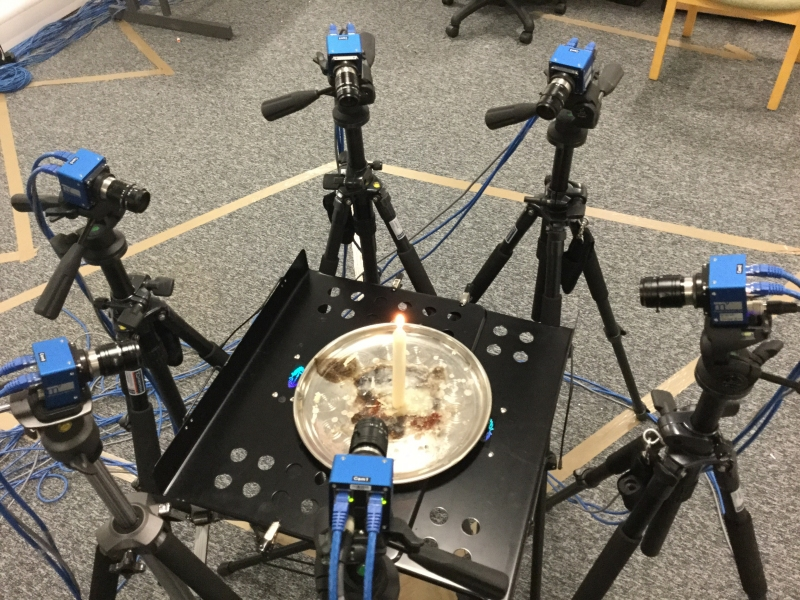
\includegraphics[width=0.8\textwidth]{img/system1}
\caption*{\tiny{Fire capture system}}
\end{figure}

\end{frame}

\begin{frame}{Pipeline}

\begin{table}[]
\centering
\begin{tabular}{|c|c|c|c|c|}
\cline{1-1} \cline{3-3} \cline{5-5}
{\bf Capture} & \multirow{3}{*}{ \raisebox{-15\totalheight}{$\rightarrow$}} & {\bf Processing} & \multirow{3}{*}{ \raisebox{-15\totalheight}{$\rightarrow$}} & {\bf Visualization} \\ \cline{1-1} \cline{3-3} \cline{5-5} 
Raw data      &                   & Refined data        &                   & Image      \\ \cline{1-1} \cline{3-3} \cline{5-5} 
\multicolumn{1}{|c|}{\raisebox{-0.95\height}{ 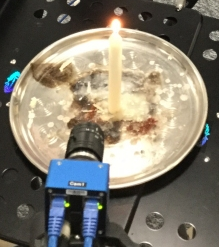
\includegraphics[width=0.22\textwidth]{img/capture_small}}} &                   & \multicolumn{1}{c|}{\raisebox{-0.95\height}{ 
\includegraphics[width=0.22\textwidth]{img/black_box}}} &                   & \multicolumn{1}{c|}{\raisebox{-0.89\height}{ 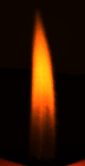
\includegraphics[width=0.15\textwidth]{img/pipelie_result}}} \\ \cline{1-1} \cline{3-3} \cline{5-5}
\end{tabular}
\end{table}

%\framebox{Capture} $\rightarrow$ \framebox{Processing} $\rightarrow$ \framebox{Visualization}  

\end{frame}

\begin{frame}{Volume rendering area}

\begin{figure}[b!]
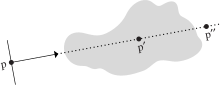
\includegraphics[width=0.8\textwidth]{img/ray_marching}
\caption*{\tiny{Diagram of light observed at $p$, image courtesy of~\cite{Pharr:2004}}}
\end{figure}

\end{frame}

\begin{frame}{The problem}

\begin{multicols}{2}

\begin{itemize}
\setlength\itemsep{0.5em}
\item Render fire realistically 
		\begin{itemize}
		\setlength\itemsep{0.5em}
		\item Participating media 
		\item Emission is important
		\item Varied fuel types
		\end{itemize}
\end{itemize}

\begin{figure}[t!]
\begin{center}
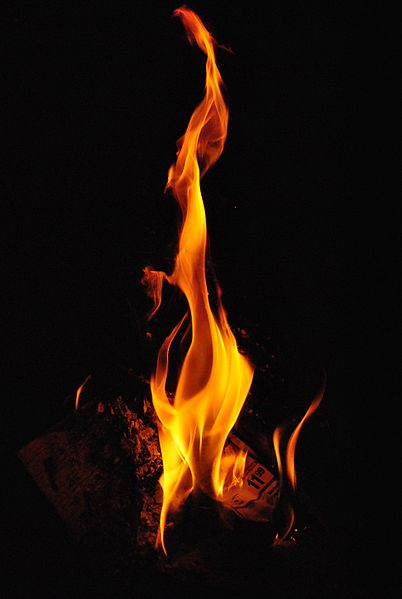
\includegraphics[width=0.3\textwidth]{img/real_fire1} 
\caption*{\tiny{Real fire with paper as fuel, image courtesy of~\cite{real_fire1}.}}
\end{center}
\end{figure}
\end{multicols}

\end{frame}

\begin{frame}{The problem: Our set-up}

\begin{multicols}{2}

\begin{itemize}
\setlength\itemsep{0.5em}
\item Fire video capture
\item Reconstruction
		\begin{itemize}
		\setlength\itemsep{0.5em}
		\item Edition
		\end{itemize}
\item Render
\end{itemize}

\begin{figure}[t!]
\begin{center}
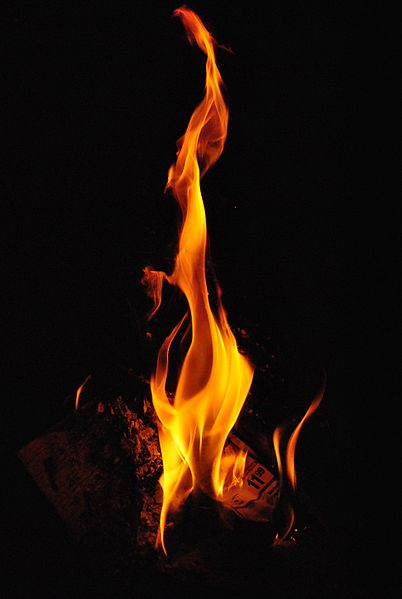
\includegraphics[width=0.3\textwidth]{img/real_fire1} 
\caption*{\tiny{Real fire with paper as fuel, image courtesy of~\cite{real_fire1}.}}
\end{center}
\end{figure}
\end{multicols}


\end{frame}

\begin{frame}{Previous work}

\begin{multicols}{2}

\begin{itemize}
\setlength\itemsep{0.5em}
\item Ray-tracing-based
		\begin{itemize}
		\setlength\itemsep{0.5em}
		\item Physically based 
		\item Accurate
		\item Slow
		\end{itemize}
\item Raster-based
		\begin{itemize}
		\setlength\itemsep{0.5em}
		\item Many artefacts
		\item Fast
		\end{itemize}
\end{itemize}


\end{multicols}


\end{frame}

\begin{frame}{Previous work: Results}

\begin{figure}[t!]
\begin{center}
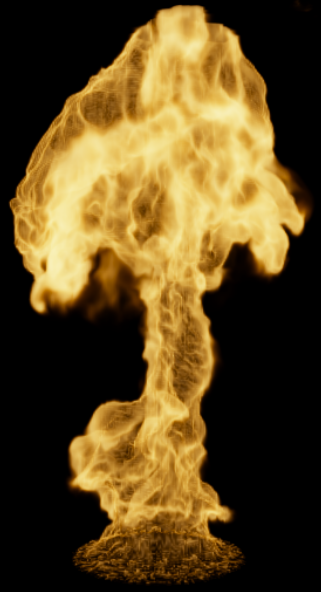
\includegraphics[width=0.3\textwidth]{img/pegoraro_2006} 
~
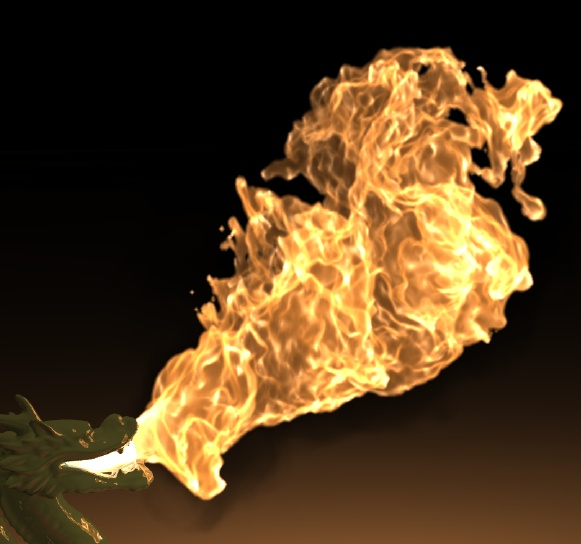
\includegraphics[width=0.59\textwidth]{img/hong_2007}
\caption*{\tiny{Left, methane fire pool~\cite{Pegoraro:2006}; right, a dragon emits a flame~\cite{Hong:2007}.}}
\end{center}
\end{figure}

\end{frame}

\section{Methodology}
\subsection{ }

\begin{frame}{The model: RTE}

\only<1,6,7>{
\begin{equation*}
(\nabla) L_{\x} = - \sigma_a L_{\x} + \sigma_a L_e - \sigma_s L_{\x} + \sigma_s \int L_{\x} \Phi d \omegam_i,
\end{equation*}
}

\only<2>{
\begin{equation*}
\boxed{ (\nabla) L_{\x}} = - \sigma_a L_{\x} + \sigma_a L_e - \sigma_s L_{\x} + \sigma_s \int L_{\x} \Phi d \omegam_i,
\end{equation*}
\vfill
Differential of radiance over a segment}

\only<3>{
\begin{equation*}
(\nabla) L_{\x} = - \boxed{\sigma_a} L_{\x} + \boxed{\sigma_a} L_e - \boxed{\sigma_s} L_{\x} + \boxed{\sigma_s} \int L_{\x} \Phi d \omegam_i,
\end{equation*}
\vfill
Absorption and scattering}

\only<4>{
\begin{equation*}
(\nabla) L_{\x} = - \sigma_a L_{\x} + \sigma_a \boxed{L_e} - \sigma_s L_{\x} + \sigma_s \int L_{\x} \Phi d \omegam_i,
\end{equation*}
\vfill
Emitted light}

\only<5>{
\begin{equation*}
(\nabla) L_{\x} = - \sigma_a L_{\x} + \sigma_a L_e - \sigma_s L_{\x} + \sigma_s \int L_{\x} \boxed{\Phi} d \omegam_i,
\end{equation*}
\vfill
Scattering function}

\only<6>{
Analytical solution

\begin{equation*}
\begin{split}
L_{\x} &= e^{-\sigma_t \deltax} L_{\x + \Delta\x} + 
 \left(1 - e^{-\sigma_t \deltax} \right) \frac{\sigma_a L_e + \sigma_s \int L_{\x} \Phi d \omegam_i}{\sigma_t}, \\
 \sigma_t &= \sigma_a + \sigma_s.
\end{split}
\end{equation*}}

\only<7>{
Analytical solution

\begin{equation*}
L_{\x} = e^{-\sigma_t \deltax} L_{\x + \boxed{\Delta\x}} + 
 \left(1 - e^{-\sigma_t \deltax} \right) \frac{\sigma_a L_e + \sigma_s \int L_{\x} \Phi d \omegam_i}{\sigma_t},
\end{equation*}
\vfill
Segment increment}

\end{frame}

\begin{frame}{The model: Important quantities}

\begin{itemize}
\setlength\itemsep{0.5em}
\item Scattering function $\Rightarrow \Phi$
\item Fuel type $\Rightarrow \sigma_a$, $\sigma_s$
	\begin{itemize}
	\setlength\itemsep{0.5em}
	\item Burning soot emission (Propane, Methane, ...)
	\item Exotic chemicals (Copper, Lithium, ...)
	\end{itemize}
\item Black Body radiation $\Rightarrow L_e$
\item Refraction $\Rightarrow \Delta\x$
\item Visual Adaptation $\Rightarrow L_{\x}$
\end{itemize}

\end{frame}

\section{Implementation}
\subsection{ }

\begin{frame}{Prior simplifications}

\only<+>{
\begin{equation*}
L_{\x} = e^{-\sigma_t \deltax} L_{\x + \Delta\x} + 
 \left(1 - e^{-\sigma_t \deltax} \right) \frac{\sigma_a L_e + \sigma_s \int L_{\x} \Phi d \omegam_i}{\sigma_t}
\end{equation*}}

\only<+>{
\begin{equation*}
\begin{split}
L_{\x} &= e^{-\sigma_t \deltax} L_{\x + \Delta\x} + 
 \left(1 - e^{-\sigma_t \deltax} \right) \frac{\sigma_a L_e + \sigma_s \int L_{\x} \Phi d \omegam_i}{\sigma_t}, \\
 \sigma_a &= 0.
\end{split}
\end{equation*}}

\only<+>{
\begin{equation*}
L_{\x} = e^{-\sigma_t \deltax} L_{\x + \Delta\x} + 
 \left(1 - e^{-\sigma_t \deltax} \right) \frac{\xcancel{\sigma_a} L_e + \xcancel{\sigma_s \int L_{\x} \Phi d \omegam_i}}{\xcancel{\sigma_t}}
\end{equation*}}

\only<+>{
\begin{equation*}
\begin{split}
&L_{\x} = e^{-\sigma_a \deltax} L_{\x + \Delta\x} + 
 \left(1 - e^{-\sigma_a \deltax} \right)  L_e \\ \\
& \mbox{Constant refraction indices}
\end{split}
\end{equation*}}

\end{frame}

\begin{frame}{Implementation overview}

\begin{multicols}{2}
\begin{itemize}
\setlength\itemsep{0.5em}
\item MentalRay shader in Maya
	\begin{itemize}
	\setlength\itemsep{0.5em}
	\item Ray marching divides the RTE into
		\begin{itemize}
		\setlength\itemsep{0.5em}
		\item Light Ray $\rightarrow L_e$
		\item Shadow Ray $\rightarrow e^{-\sigma_a \deltax} L_{\x + \Delta\x}$
		\item Eye Ray $\rightarrow L_{\x} = e^{-\sigma_a \deltax} L_{\x + \Delta\x} + L_e$
		\end{itemize}
	\item Light shader
	\item Volume/Shadow shader
	\item Utility scripts		
	\end{itemize}
\end{itemize}

\begin{figure}[t!]
\begin{center}

\includegraphics[width=0.4\textwidth]{img/mental_ray_model} 
\caption*{\tiny{Rays diagram for a sample intersection point.}}
\end{center}
\end{figure}
\end{multicols}

\end{frame}

\begin{frame}{Other details}

\begin{itemize}
\setlength\itemsep{0.5em}
\item OpenVDB $\rightarrow$ sparse voxel data
\item Uintah $\rightarrow$ fire simulation data
\item Nist $\rightarrow$ atomic spectra
\item von Kries transformation $\rightarrow$ visual adaptation
\end{itemize}

\end{frame}

\section{Results and Conclusion}
\subsection{ }

\begin{frame}[allowframebreaks]{Results}

\begin{figure}[p]
\begin{center}
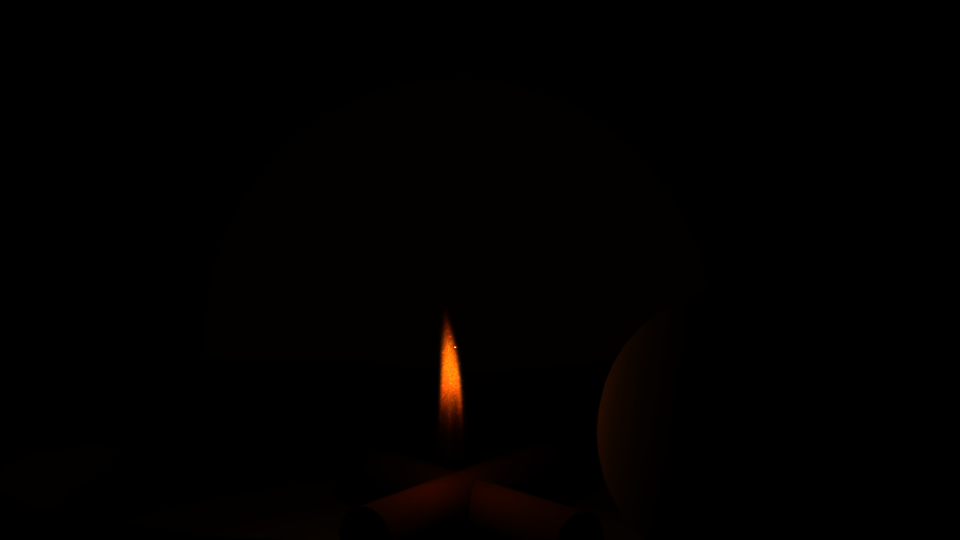
\includegraphics[width=\textwidth]{img/camp_fire_samples_64} 
\caption*{\tiny{Flame in a camp-fire.}}
\end{center}
\end{figure}

\begin{figure}[p]
\begin{center}
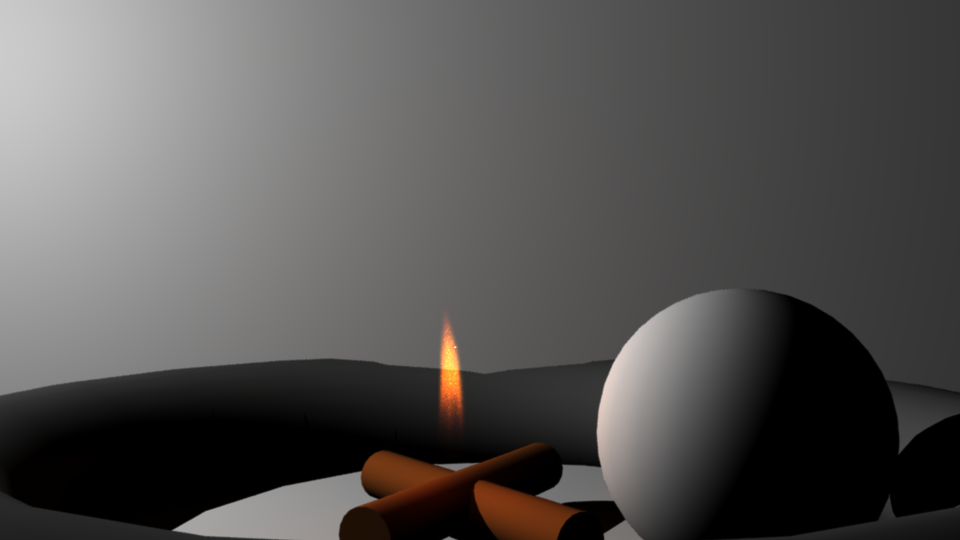
\includegraphics[width=\textwidth]{img/camp_fire_extra_light_samples_64_with_shadow_rays} 
\caption*{\tiny{Flame in a camp-fire with external light.}}
\end{center}
\end{figure}

\begin{figure}[p]
\begin{center}
\includegraphics[width=0.9\textwidth]{img/voxframe00087_max_quality_t_1200_o_250_i_3_001} 
\caption*{\tiny{Left rendered image, right ground truth.}}
\end{center}
\end{figure}

\begin{figure}[p]
\begin{center}
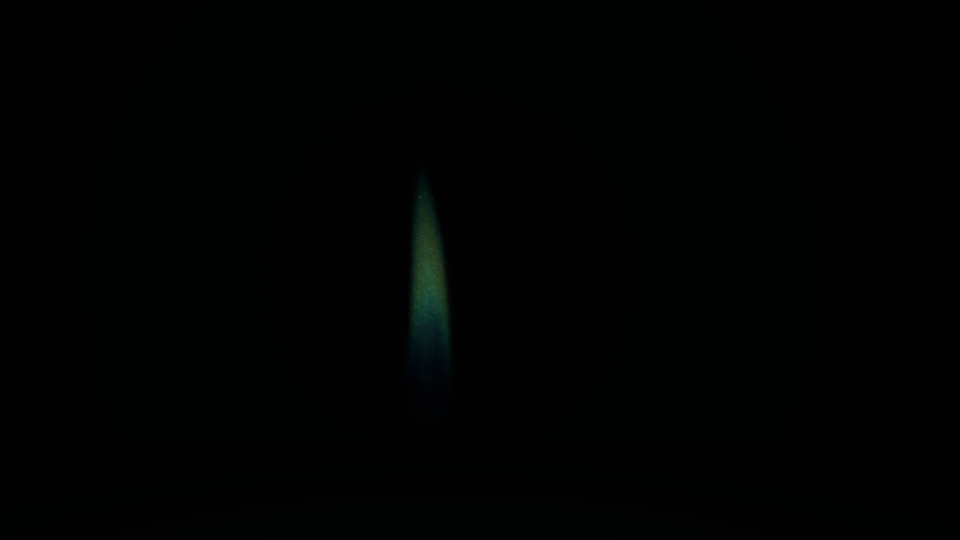
\includegraphics[width=0.9\textwidth]{img/copper_flame} 
\caption*{\tiny{Data with a new fuel.}}
\end{center}
\end{figure}


\end{frame}

\begin{frame}{Conclusions and Future Work}

\begin{itemize}
\setlength\itemsep{0.5em}
\item Limitations
	\begin{itemize}
	\setlength\itemsep{0.5em}
	\item Difficult parametrization
	\item Relies on tabulated data
	\item Computationally intensive
	\item Spherical particles
	\end{itemize}
\item Future work
	\begin{itemize}
	\setlength\itemsep{0.5em}
	\item Importance sampling
	\item Automatic parameter estimation
	\end{itemize}
\end{itemize}

\end{frame}

\begin{frame}{Parameter Estimation}

\begin{itemize}
\setlength\itemsep{0.5em}
\item Spectrum reconstruction
\item Under constrained
\item Prior knowledge
	\begin{itemize}
	\setlength\itemsep{0.5em}
	\item Camera sensitivity
	\end{itemize}
\item Previous work,~\cite{Smits:1999},~\cite{Sun2001},~\cite{Drew:2003}
\end{itemize}

\end{frame}

\section*{}

\begin{frame}[plain,c]

\begin{center}
\huge Thank you
\\~\\
\Large Questions?
\end{center}

\end{frame}


\begin{frame}[allowframebreaks]{References}

\bibliographystyle{apalike}
\bibliography{bibliography}

\end{frame}

\section{Live demo}


%----------------------------------------------------------------------

\end{document}
